\begin{apendicesenv}

\partapendices

\chapter{Conector API de Gerenciamento de Usuários}

\begin{figure}[!hbt]
\centering
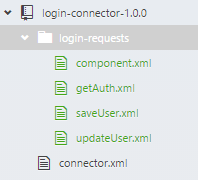
\includegraphics[scale=1]{figuras/estrutura_conector_login.png}
\caption{Estrutura de pacotes do conector criado para a API de gerenciamento de usuários.}
\end{figure}


\definecolor{verde}{rgb}{0.25,0.5,0.35}
\definecolor{jpurple}{rgb}{0.5,0,0.35}

\lstset{
  language=XML,
  basicstyle=\ttfamily\small, 
  keywordstyle=\color{jpurple}\bfseries,
  stringstyle=\color{blue},
  commentstyle=\color{verde},
  extendedchars=true, 
  showspaces=false, 
  showstringspaces=false, 
  numbers=left,
  numberstyle=\tiny,
  breaklines=true, 
  backgroundcolor=\color{cyan!10}, 
  breakautoindent=true, 
  captionpos=b,
  xleftmargin=0pt,
  tabsize=4,
  texcl=true
}
\begin{lstlisting}[caption={Conteúdo do arquivo "connector.xml".}]
<?xml version="1.0" encoding="UTF-8"?>
<connector>
    <component name="login" package="org.wso2.carbon.connector" >
		<dependency component="login-requests"/>
        <description>Login API connector libraries.</description>
    </component>
</connector>
\end{lstlisting}


\definecolor{verde}{rgb}{0.25,0.5,0.35}
\definecolor{jpurple}{rgb}{0.5,0,0.35}

\lstset{
  language=XML,
  basicstyle=\ttfamily\small, 
  keywordstyle=\color{jpurple}\bfseries,
  stringstyle=\color{blue},
  commentstyle=\color{verde},
  extendedchars=true, 
  showspaces=false, 
  showstringspaces=false, 
  numbers=left,
  numberstyle=\tiny,
  breaklines=true, 
  backgroundcolor=\color{cyan!10}, 
  breakautoindent=true, 
  captionpos=b,
  xleftmargin=0pt,
  tabsize=4,
  texcl=true
}
\begin{lstlisting}[caption={Conteúdo do arquivo "component.xml".}]
<?xml version="1.0" encoding="UTF-8"?>
<component name="login-requests" type="synapse/template">
    <subComponents>
        <component name="getAuth">
            <file>getAuth.xml</file>
            <description>
                Check if user is registered and authorized to access the client application.
            </description>
        </component>url = "http://localhost:8001/users/"
        <component name="saveUser">
            <file>saveUser.xml</file>
            <description>
                Save a user instance associated to a client application.
            </description>
        </component>
        <component name="updateUser">
            <file>updateUser.xml</file>
            <description>
                Update user instance indicated by the client application.
            </description>
        </component>
    </subComponents>
</component>
\end{lstlisting}


\definecolor{verde}{rgb}{0.25,0.5,0.35}
\definecolor{jpurple}{rgb}{0.5,0,0.35}

\lstset{
  language=XML,
  basicstyle=\ttfamily\small, 
  keywordstyle=\color{jpurple}\bfseries,
  stringstyle=\color{blue},
  commentstyle=\color{verde},
  extendedchars=true, 
  showspaces=false, 
  showstringspaces=false, 
  numbers=left,
  numberstyle=\tiny,
  breaklines=true, 
  backgroundcolor=\color{cyan!10}, 
  breakautoindent=true, 
  captionpos=b,
  xleftmargin=0pt,
  tabsize=4,
  texcl=true
}
\begin{lstlisting}[caption={Conteúdo do arquivo "getAuth.xml".}]
<?xml version="1.0" encoding="UTF-8"?>
<template name="getAuth" xmlns="http://ws.apache.org/ns/synapse">
    <parameter name="username" description="O username do usuario (valor unico)."/>
    <parameter name="client_name" description="Nome identificador da aplicacao cliente"/>
    <sequence>
        <property name="uri.var.username" expression="$func:username"/>
        <property name="uri.var.client_name" expression="$func:client_name"/>
        <call>
            <endpoint>
                <http method="get"
                      uri-template="http://localhost:8001/users/username={uri.var.username}&amp;aplicacao={uri.var.client_name}"/>
            </endpoint>
        </call>
    </sequence>
</template>
\end{lstlisting}


\definecolor{verde}{rgb}{0.25,0.5,0.35}
\definecolor{jpurple}{rgb}{0.5,0,0.35}

\lstset{
  language=XML,
  basicstyle=\ttfamily\small, 
  keywordstyle=\color{jpurple}\bfseries,
  stringstyle=\color{blue},
  commentstyle=\color{verde},
  extendedchars=true, 
  showspaces=false, 
  showstringspaces=false, 
  numbers=left,
  numberstyle=\tiny,
  breaklines=true, 
  backgroundcolor=\color{cyan!10}, 
  breakautoindent=true, 
  captionpos=b,
  xleftmargin=0pt,
  tabsize=4,
  texcl=true
}
\begin{lstlisting}[caption={Conteúdo do arquivo "saveUser.xml".}]
<?xml version="1.0" encoding="UTF-8"?>
<template name="saveUser" xmlns="http://ws.apache.org/ns/synapse">
    <parameter name="aplicacao" description="Nome da aplicacao cliente a qual o usuario esta associado."/>
    <parameter name="username" description="Dados do usuario a ser salvo. Nome de usuario."/>
    <parameter name="password" description="Dados do usuario a ser salvo. Senha."/>
    <parameter name="first_name" description="Dados do usuario a ser salvo. Primeiro nome."/>
    <parameter name="last_name" description="Dados do usuario a ser salvo. Ultimo nome."/>
    <parameter name="email" description="Dados do usuario a ser salvo. Email nome."/>
    <sequence>

        <property name="uri.var.aplicacao" expression="json-eval($.aplicacao)"/>
        <property name="uri.var.username" expression="json-eval($.username)"/>
        <property name="uri.var.password" expression="json-eval($.password)"/>
        <property name="uri.var.first_name" expression="json-eval($.first_name)"/>
        <property name="uri.var.last_name" expression="json-eval($.last_name)"/>
        <property name="uri.var.email" expression="json-eval($.email)"/>


        <payloadFactory media-type="json">
            <format>
                {"usuario":{"username":"$1","password":"$2","first_name":"$3","last_name":"$4","email":"$5"}, "aplicacao":"$6"}
            </format>
                  <args>
                     <arg evaluator="json" expression="$.username"/>
                     <arg evaluator="json" expression="$.password"/>
                     <arg evaluator="json" expression="$.first_name"/>
                     <arg evaluator="json" expression="$.last_name"/>
                     <arg evaluator="json" expression="$.email"/>
                     <arg evaluator="json" expression="$.aplicacao"/>
                  </args>
        </payloadFactory>

        <property name="messageType" value="application/json" scope="axis2" type="STRING"/>
        <property name="content-type" value="application/json" scope="axis2" type="STRING"/>
        <property name="DISABLE_CHUNKING" scope="axis2" value="true"/>

        <log level="full"/>
            <call>
                <endpoint>
                    <http method="post"
                          uri-template="http://localhost:8001/users/"/>
                </endpoint>
            </call>
    </sequence>
</template>
\end{lstlisting}

\definecolor{verde}{rgb}{0.25,0.5,0.35}
\definecolor{jpurple}{rgb}{0.5,0,0.35}

\lstset{
  language=XML,
  basicstyle=\ttfamily\small, 
  keywordstyle=\color{jpurple}\bfseries,
  stringstyle=\color{blue},
  commentstyle=\color{verde},
  extendedchars=true, 
  showspaces=false, 
  showstringspaces=false, 
  numbers=left,
  numberstyle=\tiny,
  breaklines=true, 
  backgroundcolor=\color{cyan!10}, 
  breakautoindent=true, 
  captionpos=b,
  xleftmargin=0pt,
  tabsize=4,
  texcl=true
}
\begin{lstlisting}[caption={Conteúdo do arquivo "saveUser.xml".}]
<?xml version="1.0" encoding="UTF-8"?>
<template name="updateUser" xmlns="http://ws.apache.org/ns/synapse">
    <parameter name="username" description="Dados do usuario a ser salvo. Nome de usuario."/>
    <parameter name="password" description="Dados do usuario a ser salvo. Senha."/>
    <parameter name="first_name" description="Dados do usuario a ser salvo. Primeiro nome."/>
    <parameter name="last_name" description="Dados do usuario a ser salvo. Ultimo nome."/>
    <parameter name="email" description="Dados do usuario a ser salvo. Email nome."/>
    <sequence>
        <property name="uri.var.username" expression="$func:username"/>
        <property name="uri.var.password" expression="$func:password"/>
        <property name="uri.var.first_name" expression="$func:first_name"/>
        <property name="uri.var.last_name" expression="$func:last_name"/>
        <property name="uri.var.email" expression="$func:email"/>

        <payloadFactory media-type="json">
            <format>
                {"username":"$1","password":"$2","first_name":"$3","last_name":"$4","email":"$5"}
            </format>
            <args>
                <arg evaluator="json" expression="$.username"/>
                <arg evaluator="json" expression="$.password"/>
                <arg evaluator="json" expression="$.first_name"/>
                <arg evaluator="json" expression="$.last_name"/>
                <arg evaluator="json" expression="$.email"/>
            </args>
        </payloadFactory>

        <property name="contentType" value="application/json" scope="axis2" type="STRING"/>
        <property name="messageType" scope="axis2" value="application/json" type="STRING"/>
        <property name="DISABLE_CHUNKING" scope="axis2" value="true"/>

        <log level="full"/>

        <call>
            <endpoint>
                <http method="put"
                      uri-template="http://localhost:8001/users/username={+uri.var.username}"/>
            </endpoint>
        </call>
    </sequence>
</template>
\end{lstlisting}

%\chapter{Segundo Apêndice}

%Texto do segundo apêndice.

\end{apendicesenv}
